\section{Processor Emulation}

To emulate the sub-threshold ARM Cortex M0+ two possible methods were considered. The first was to obtain verilog code of a similar processor and run it upon an FPGA. The verilog code could potentially then be altered to provide the same constraints as the sub-threshold device. The other method considered was to obtain a development board which uses a similar processor. Upon this, to emulate the sub-threshold device, the system clock frequency can be reduced and closer attention paid to the binary uploaded and the memory it would use.

The two processors considered for this were the ARM Cortex M0 and M0+, however the M0+ was quickly dismissed due to the lack of accessibility to verilog code which was available for the M0 via ARMs Design Start. The accessibility of development boards was not found to be an issue, as boards were found containing both processors. 

\namedsubsection{ARM Cortex M0 Processor \label{sec:cortex}}{Pasat}

This section discusses one of the main requirements and one of the essential aspects of the project: using ARM's Cortex M0 processor. This processor is a member of the Cortex-M family and offers a great tradeoff between costs and performance/functionality. It has been designed in order to allow intelligent compromises in terms of power usage, computational power and in the simplicity of the design. It implements a simplified version of the Advanced Microcontroller Bus Architecture (AMBA), the AMBA-Lite Bus, which allows connection to different peripherals. In this way, the Cortex-M0 generally acts as the master device and the peripherals act as slaves. In figure \ref{fig:cortexm0ds}, the schematic for the processor can be seen.\\
\begin{figure}
\centering
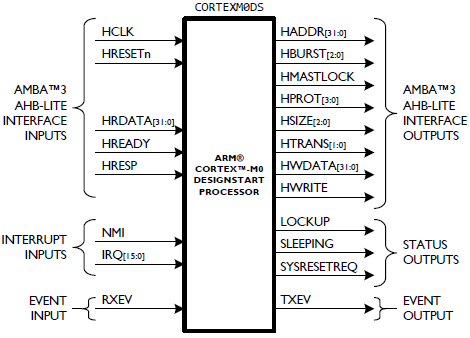
\includegraphics[scale=0.7]{figures/cortexm0ds_schematic.PNG}
\caption{Cortex M0DS schematic \cite{armdesignstart}} \label{fig:cortexm0ds}
\end{figure}
\clearpage

\begin{figure}
\centering
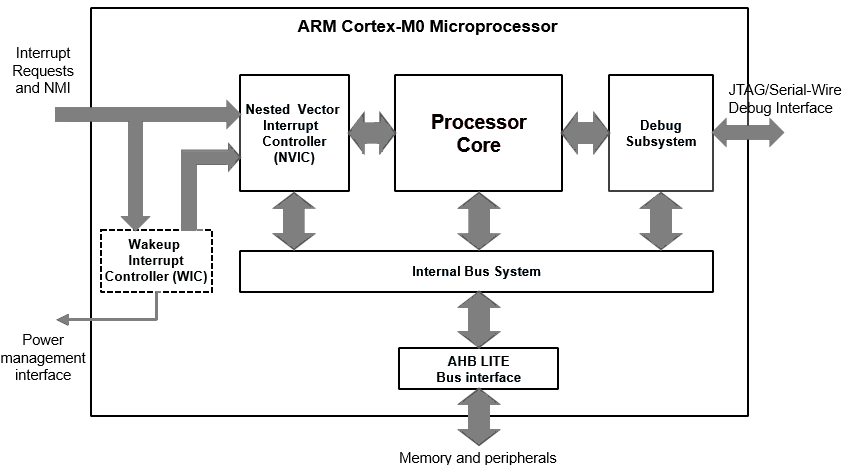
\includegraphics[scale=0.7]{figures/arm_cortexm0_microprocessor.PNG}
\caption{Cortex-M0 Block Diagram \cite{armdesignstart}} \label{fig:cortex_block}
\end{figure}

The Cortex M0 has a 32-bit reduced instruction set computing (RISC) processor. It uses the ARMv6-M(Microcontroller), which is a subset of the ARMv7-M profile but includes fewer instructions. The Cortex M0 is based on a Von-Neumann architecture, having both data and instructions share a single bus interface. It provides a Debug Extension that includes some architectural extensions to support debugging. The ARMv6-M offers support for 56 instructions as a subset of  Thumb-1(16-bit) and Thumb-2(16/32b-bit) which are present in the ARMv6T2. The Cortex M0 block diagram can be seen above in figure \ref{fig:cortex_block}. 

The Processor Core contains the internal registers, data path, ALU and control logics. The Cortex M0 has a three-stage pipeline: fetch, decode and exection and includes the 32-bit registers for general and special usages. The Cortex M0+ has only a two-stage pipeline to reduce the power usage.

The Nested Vectored Interrupt Controller (NVIC) handles up to 32 interrupts request signals and one NMI (Non-Maskable Interrupt). It also fulfils tasks such as comparing priorities between  interrupt requests and the current priority level. 

The Bus system contains the internal bus system, the data path in the processor core and the AHB LITE interface unit which is an on-chip bus protocol which enables some features required for high-performance, high clock frequency systems. 

The Debug system handles the program breakpoints, debugging control and the data watchpoints. This can put the processor in a  static state in order for the programmer to evaluate and analyse the status of the processor in that specific moment.

The Wakeup Interrupt Controller (WIC) is important for this project because it is used in low-power applications. The microcontroller can be set to enter sleep mode by turning off most of its components. If a interrupt request is sent, this component can inform the unit that handles the power management to power up the system.

\subsubsection{Limitations \label{sec:cortex-limitations}}

One of the major challenges which was encountered in the use of the Cortex M0 is the lack of hardware division or floating point unit. To account for this, there are software libraries which perform these operations however, they can take quite a large number of cycles to perform and hence would be impractical on a constrained system.

Since the Cortex M0 is such a low-power, lost-cost device, it comes with its limitations. The device only offers 32kB on-chip flash programming memory and only 8kB SRAM. Basic applications have been developed for this processor, but in order to allow the implementation of a more complex program, such as exercise recognition, the code and libraries need to be very well optimised. All the unnecessary functionalities available in libraries must be disposed in order to save memory on this constrained system.
\namedsubsection{FPGA}{Pasat}

An Field-Programmable Gate Array (FPGA) is a semiconductor device which is has a matrix of Configurable Logic Blocks (CLB) connected through programmable interconnects. One main advantage of the FPGA is that it can be preprogrammed after they are manufactured in order to fit desired functionalities and requirements. Interesting projects have also been realized with this processor on a FPGA, such as advanced real traffic light controller \cite{traffic_light}.

Typically, the FPGA differs great from the conventional microcontroller; the microcontroller has the chip already designed. The programmer simply writes the software in C or C++, then it is compiled into a hex file that is loaded on the microcontroller. The program is stored in the flash memory until is is replaced or erased.

FPGAs are different in this sense. The circuit is completely designed by the programmer. The processor must be created and can be as simple as an and gate or can be our Cortex M0+. HDL is used to write the design, which is then synthesized into a bit file which configures the FPGA. One small problem with this is the fact that it stores the configuration in the RAM, so once the power is gone, the configuration is lost.

The board used for this project is the Xilinx Digilent Nexys4, which can be seen in figure \ref{fig:nexys4}. It is based on the Artix-7 which has a low power consumption and cost \cite{cortexm0onnexys4}. Implementations were also successful on low end FPGAs. This board was chosen because it is a large, high-capacity FPGA board that would be sufficient for our project. Another reason is the fact that is has several built in peripherals, such as accelerometer, which would be useful for the exercise detection. 

\begin{figure}
\centering
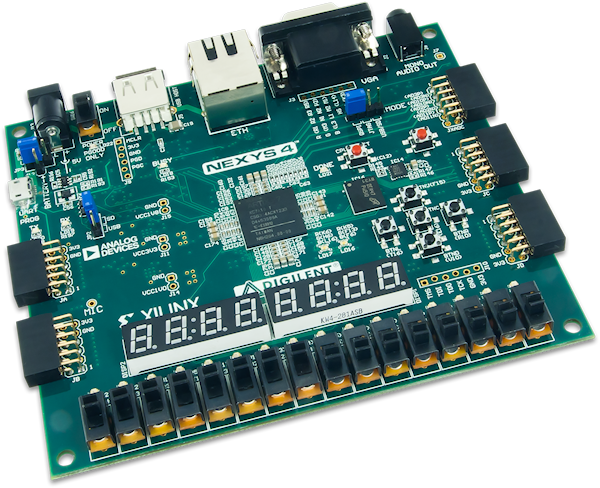
\includegraphics[scale=0.7]{figures/nexys4.PNG}
\caption{Xilinx Digilent Nexys4 \label{fig:nexys4}}
\end{figure}

\namedsubsection{mBed}{Gupta}

mBed is a platform which implements ARM 32-bit processors within micro-controllers which is primarily developed by ARM. They are of the DIP form factor with 40 pins. It features an online SDK allowing for the development of projects online. It permits code to be written online as well as compiled into a binary compatible with the board being used. This binary can then be downloaded removing the pre-requisite of having the ARM toolchain available locally. The manner of uploading to the mBed is relatively straight forward with the presence of the mBed interface. \cite{mbed_website}\todo{Try expanding on this section}

This interface exposes a Mass Storage device to the host computer via a USB connection allowing for binaries to be uploaded in a drag and drop manner. The interface is also connected with the target chip using a JTAG connection allowing for it to program its flash memory. When the reset button is pressed, the interface checks the storage for the newest binary file and, should it not be programmed within the device already, will program the binary provided into the flash memory of the chip. \cite{mbed_website}\todo{Try expanding this section as well}

\subsubsection{Why the mBed}

When \todo{Need a better name for this subsection?} initially looking at various ways to emulate the sub-threshold version of the ARM Cortex M0, using an existing non sub-threshold version of the ARM Cortex M0 was considered. This involved searching for some form of micro-controller or device which would allow for programming of the processor. This lead to the mBed family which appeared easy to program and use featuring ARM processors. Within the mBed family of micro-controllers, the LPC11U24 model uses an ARM Cortex M0 as its processor.

An important factor for the device is being able to communicate with other devices using various communication protocols. Fortunately, multiple pins are broken out on the mBed which allow for flexibility in choice, in particular there are 2 SPI, 1 I2C, and 1 Serial interfaces available simultaneously upon the mBed. \cite{mbed_website} 

For obtaining data from the sensor, it is most likely to use I2C or One-Wire communication, should it be I2C, the mBed would work well. It also allows for the Serial pins to be interfaced with the host PC allowing for debugging information to be transmitted to the host PC. 

The requirements for this project require the processor to be emulate the sub-threshold version which operates with a system clock in the range of a few hundred kHz to a few MHz. This would require a clock in the micro-controller which can operate at these frequencies and also be able to be set as the system clock.

The device typically runs at 48MHz using its Internal RC oscillator (IRC) as its system clock. However, it also has the ability to switch its system clock to be sourced from the internal Watchdog oscillator instead. 

This oscillator consists of two parts, an oscillator function which generates an analog clock (\verb|Fclkana|) as well as a divisor (\verb|DIVSEL|) which is used to divide the analog clock to the required output frequency (\verb|wdt_osc_clk|). The output frequency can be calculated using Equation~\ref{eq:wdt_osc_clk} and is within the range $ 9.4 $ kHz $ \leq \verb|wdt_osc_clk| \leq 2.3 $ MHz. \cite{mbed_datasheet}

\begin{equation}
	\label{eq:wdt_osc_clk}
	\verb|wdt_osc_clk| = \frac{Fclkana}{2 * (1 + DIVSEL)}
\end{equation}

Some concerns were made realising that the Watchdog oscillator has an error margin of $\pm 40\%$ for the frequency of Fclkana. In a meeting with the client, it was decided to carry forward with the device while paying attention to this margin and analysing the impact of it upon the project.